\documentclass{oci}
\usepackage[utf8]{inputenc}
\usepackage{lipsum}

\title{Figuras}

\begin{document}
\begin{problemDescription}
Sofía ama viajar, y hoy se encuentra de viaje por la mítica ciudad de Pelotillehue.

Apasionada por la historia del lugar, investigó las leyendas más recónditas de la zona y se dirigió al Templo de Buenas Peras. En una de sus salas más enigmáticas se encuentran dos grillas de dimensiones $n \times m$: una dispuesta en la pared, dibujando una figura, y otra en el suelo, con bloques de oro en sus casillas.

Ella sabe que si logra hacer coincidir las dos figuras, se abrirá una puerta secreta al otro lado de la sala. Para esto, cuenta con una tableta mágica que le permite realizar la siguiente operación: retirar un bloque de la grilla y colocarlo adyacente a cualquier otro bloque.

Por ejemplo, supongamos que se encuentran las siguientes figuras en el piso y en la pared, respectivamente.

\begin{center}
    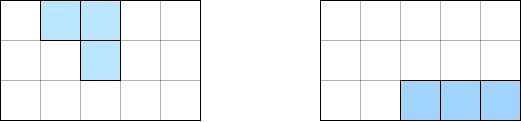
\includegraphics[scale=0.7]{figura1.png}
\end{center}

Sofía puede ejecutar la siguiente secuencia de operaciones para hacer coincidir ambas figuras.

\begin{center}
    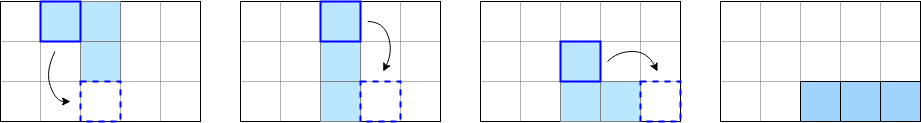
\includegraphics[scale=0.5]{figurras2.png}
\end{center}

Llena de curiosidad por descubrir lo que el templo ocultaba, Sofía intentó hacer coincidir las figuras. Lamentablemente, tras horas y horas de intentarlo, no lo logró y decidió comunicarse contigo para que le eches una mano.

Dado el diseño de las dos grillas, ¿puedes ayudar a Sofía a encontrar el número mínimo de operaciones necesarias para transformar la grilla del suelo en la grilla de la pared?

\end{problemDescription}

\begin{inputDescription}
La entrada consiste de varias líneas.\\
La primera línea contiene 2 enteros $n, m$ $(n \cdot m \leq 2 \cdot 10^5)$ representando las dimensiones de ambas grillas.\\

Las siguientes $n$ líneas consisten en $m$ caracteres representando la grilla del piso.\\

Luego siguen otras $n$ líneas de $m$ caracteres que describen la grilla de la pared.\\

Cada caracter corresponde a un $1$ si la casilla contiene un bloque o un $0$ si no.
\end{inputDescription}

\begin{outputDescription}
La salida debe contener un entero, el número mínimo de operaciones para transformar la primera grilla en la segunda. En caso de que no se pueda, imprimir "IMPOSIBLE" (sin las comillas).
\end{outputDescription}

\begin{scoreDescription}
  \subtask{20}
  Se probarán varios casos en donde el número total de $1$s en las dos grillas es menor a $10^3$.
  \subtask{50}
  Se probarán varios casos sin restricciones adicionales.
\end{scoreDescription}

\begin{sampleDescription}
\sampleIO{sample-1}
\sampleIO{sample-2}
\end{sampleDescription}

\end{document}
